\subsection{Welten}
\mysubsubsection{Lydia Friedrich}{Gebirgswelt}

\begin{figure}[!htbp]%[htbp]
	\centering
		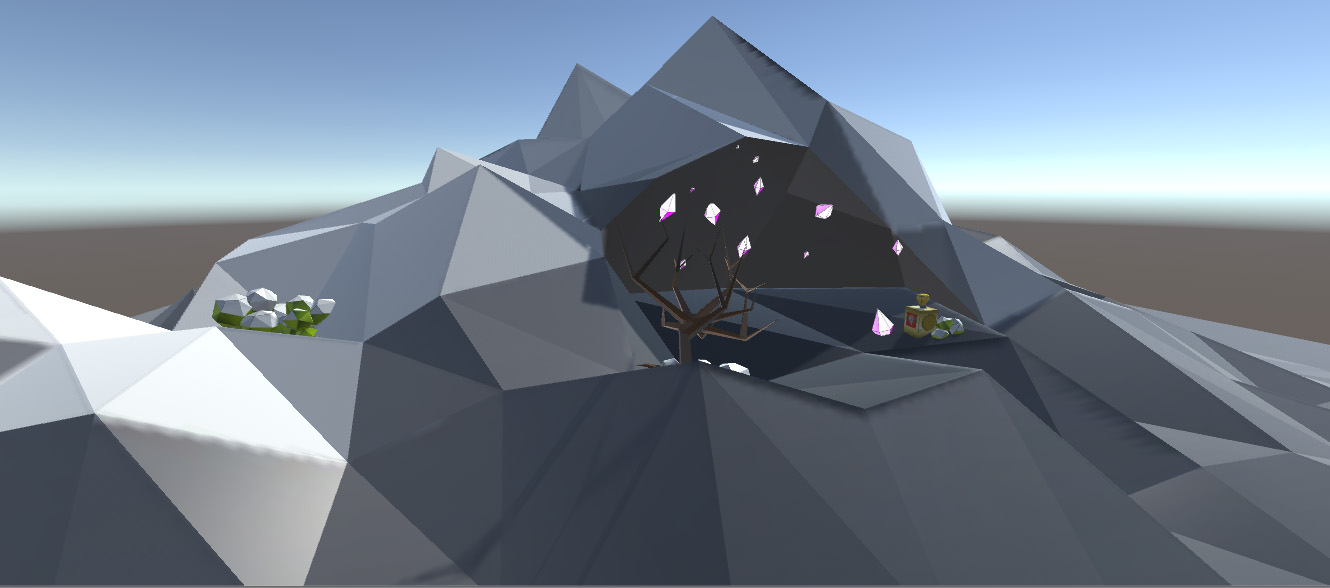
\includegraphics[width=1.0\textwidth]{images/Gebirge}
	\caption{Screenshot der Gebirgslandschaft}
	\label{fig:Gebirge}
\end{figure}

Die Gebirgswelt ist die einzige Welt, die der Nutzer zu Beginn des Spiels ansteuern und erkunden kann. Die leuchtenden Kristalle, innerhalb der Berghöhle, erzeugen in der Dunkelheit eine mysteriöse und aufregende Stimmung. Sobald der Würfel mit Licht gefüllt ist, nimmt der Spieler die Gebirgswelt erneut und sehr wahrscheinlich anders, als zuvor im Dunkeln, war. Diese Welt ist bei Tag durch einen großen Berg und den darauf lebenden Bergziegen geprägt.

\mysubsubsection{Sandra Beuck}{Dorfwelt}

\begin{figure}[!htbp]%[htbp]
	\centering
		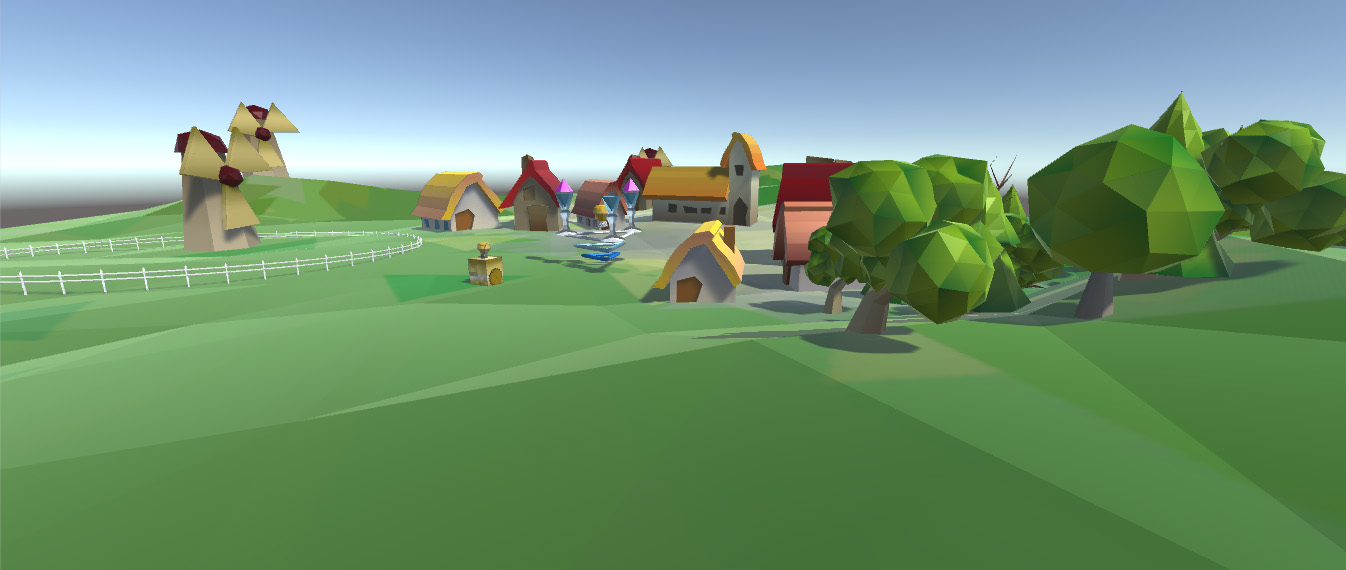
\includegraphics[width=1.0\textwidth]{images/Dorf}
	\caption{Screenshot der Dorflandschaft}
	\label{fig:Dorf}
\end{figure}

Das Dorf bietet den Bewohnern der Inselwelt ein gemütliches Zuhause. Windmühlen, kleine Häuser und viel Grünfläche, auf der Schafe grasen, wirken beruhigend und liefern dem Spieler einen angenehmen Start in das Spiel, wenn er zu Beginn die Lichtmaschine repariert. Die Farbstimmung ist fröhlich und offen gestaltet. Im Dorf gibt es einen NPC sowie weitere Dorfbewohner, die dem Spieler einiges zu entdecken geben.

\mysubsubsection{Lydia Friedrich}{Waldwelt}

\begin{figure}[!htbp]%[htbp]
	\centering
		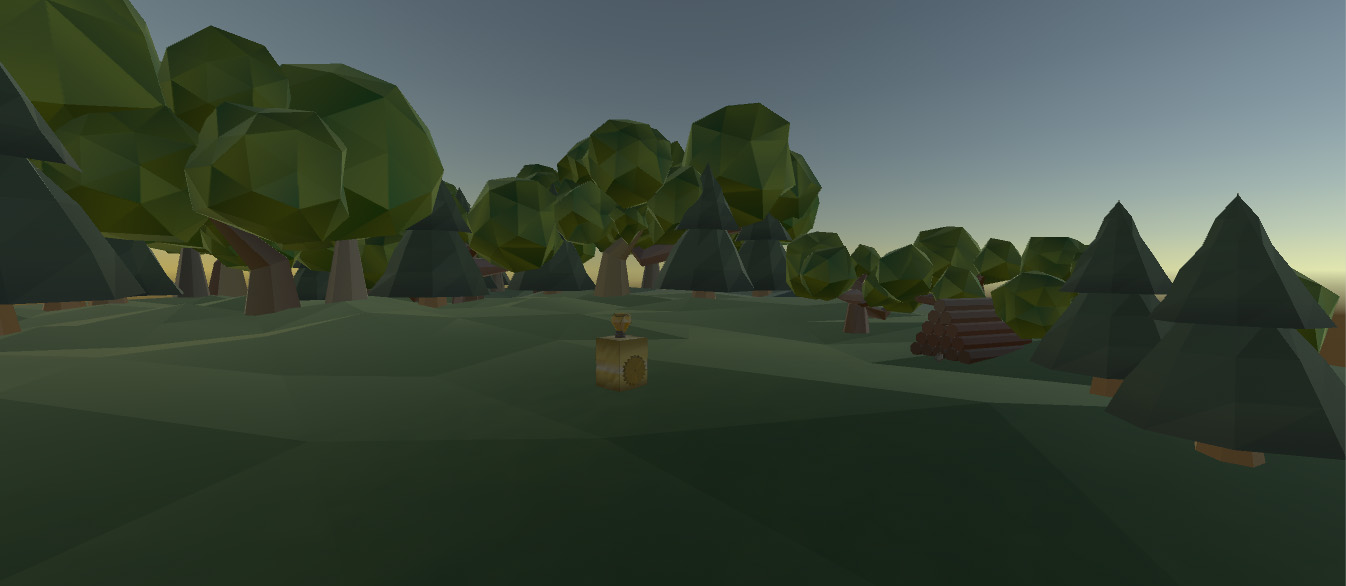
\includegraphics[width=1.0\textwidth]{images/Wald}
	\caption{Screenshot der Waldlandschaft}
	\label{fig:Wald}
\end{figure}

Diese Welt steht für das Sinnbild der Natur: der Wald. Absicht ist es, dass sich der Spieler innerhalb dieser Welt wohlfühlt. Er hat die Möglichkeit unberührte Natur zu genießen sowie Rehe in freier Wildbahn zu beobachten. Diese Welt ist durch ihren hohen Anteil an Bäumen geprägt. Der Spieler hat die Möglichkeit die Schaufel, welche an einem Holzstapel lehnt, einzusammeln.

\mysubsubsection{Sandra Beuck}{Wüstenwelt}

\begin{figure}[!htbp]%[htbp]
	\centering
		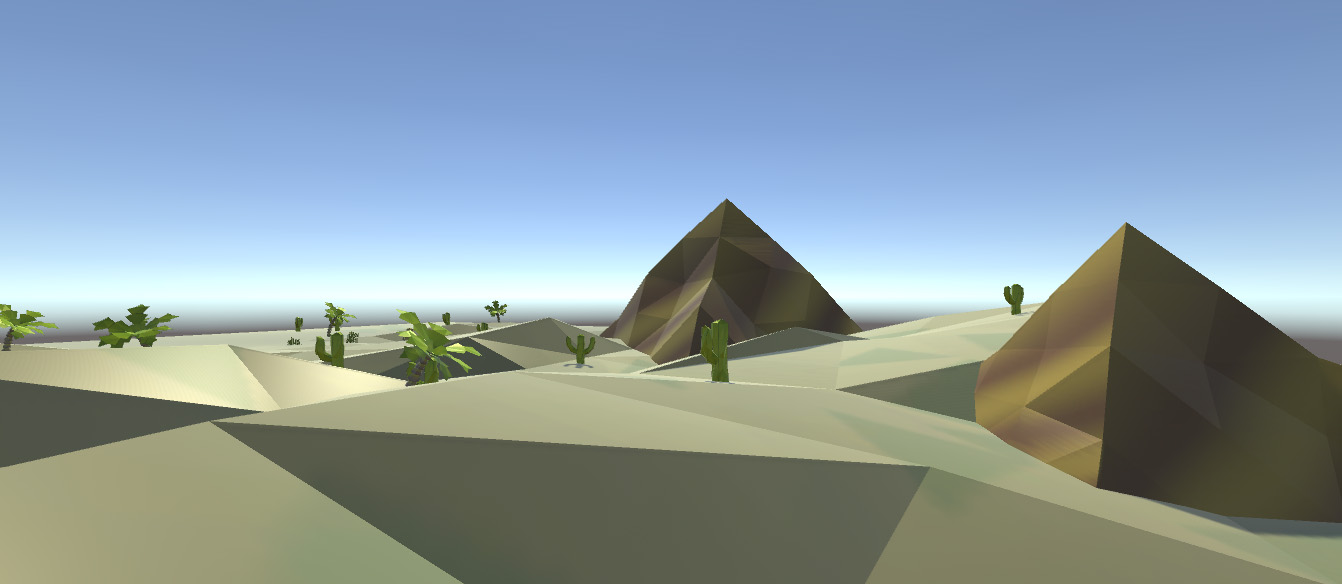
\includegraphics[width=1.0\textwidth]{images/Wueste}
	\caption{Screenshot der Wüstenlandschaft}
	\label{fig:Wueste}
\end{figure}

Die Wüste bildet den Gegensatz zum Wald. Sie wirkt weitläufig und karg auf den Spieler und ist durch Pyramiden und Dünen gezeichnet. Außer einer Schlange, die sich durch den trockenen Sand schlängelt, gibt es weder Tiere noch Menschen.
Die Farbgebung und der geringe Einsatz von Objekten unterstreicht diese Wirkung. In der Wüste befindet sich ein Teil des Würfels, den der Spieler mit Hilfe der Schaufel unter einem Sanddecken-Objekt finden kann.  

\mysubsubsection{Sandra Beuck}{Feuerwelt}

\begin{figure}[!htbp]%[htbp]
	\centering
		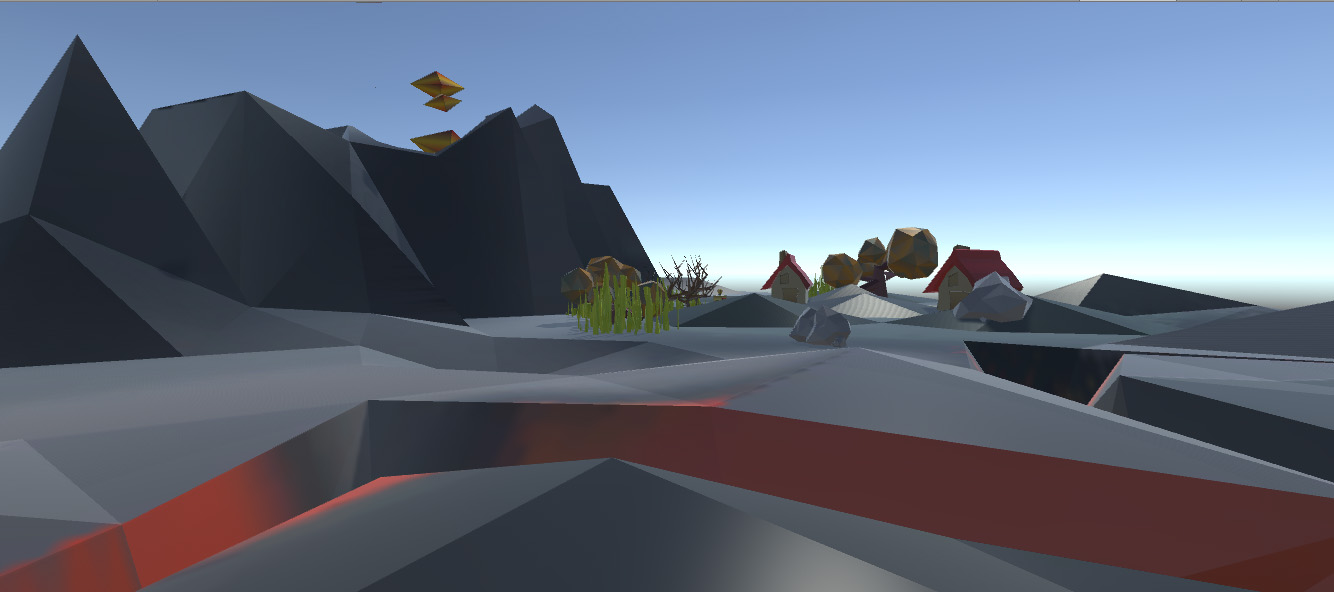
\includegraphics[width=1.0\textwidth]{images/Feuer}
	\caption{Screenshot der Feuerlandschaft}
	\label{fig:Feuer}
\end{figure}

Die Feuerwelt ist eine karge Landschaft, die von vielen Vulkanausbrüchen gezeichnet ist. Spärliche Vegetation und viele Felsen zeichnen sie aus.  Die Farben sind sehr dunkel gestaltet, so sticht die Lava des Vulkanausbruchs dem Spieler sofort ins Auge. Durch den Vulkanausbruch geht ein Haus in Flammen auf und muss gelöscht werden. Vor dem brennenden Haus ist ein NPC, mit dem der Spieler interagieren kann.

\mysubsubsection{Lydia Friedrich}{Eiswelt}

\begin{figure}[!htbp]
	\centering
		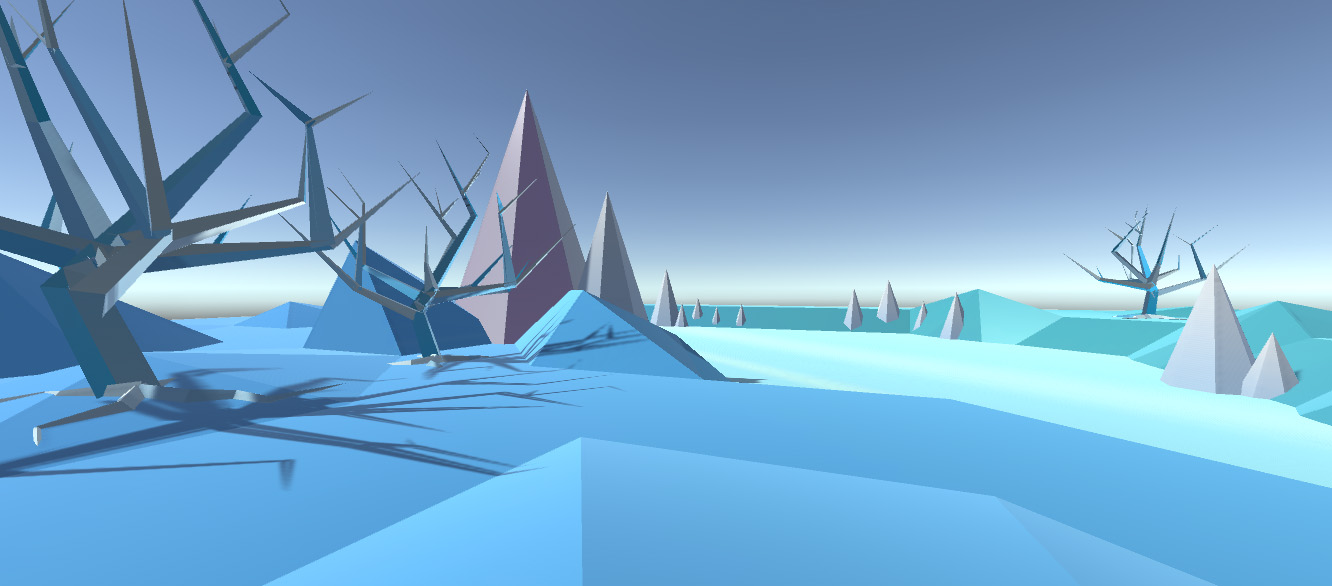
\includegraphics[width=1.0\textwidth]{images/Eis}
	\caption{Screenshot der Eislandschaft}
	\label{fig:Eis}
\end{figure}

Die Eiswelt ist die Gegensatzwelt zur Feuerwelt. Sie ist farblich sehr kühl gestaltet, damit der Spieler sich besser in die Eiswelt hineinfühlen kann. Die Landschaft ist bewusst sehr grob und weitflächig angelegt, da diese auch in der realen Welt nicht viele Möglichkeiten für Vegetationen und Lebewesen bietet. Jedoch hat sich ein Pinguin in dieser Welt nieder gelassen und dreht munter seine Runden auf der großen Eisfläche. Wichtigstes Element in dieser Welt ist der Eiszapfen, welchen der Spieler benötigt um ein brennendes Haus in der Feuerwelt zu löschen. Dieser Eiszapfen hat einen leichten rosa Schimmer. Grund dafür ist die Auffälligkeit im Gegensatz zu den anderen Eiszapfen in dieser Welt.

\mysubsubsection{Lydia Friedrich}{Skybox}

\begin{figure}[!htbp]
	\centering
		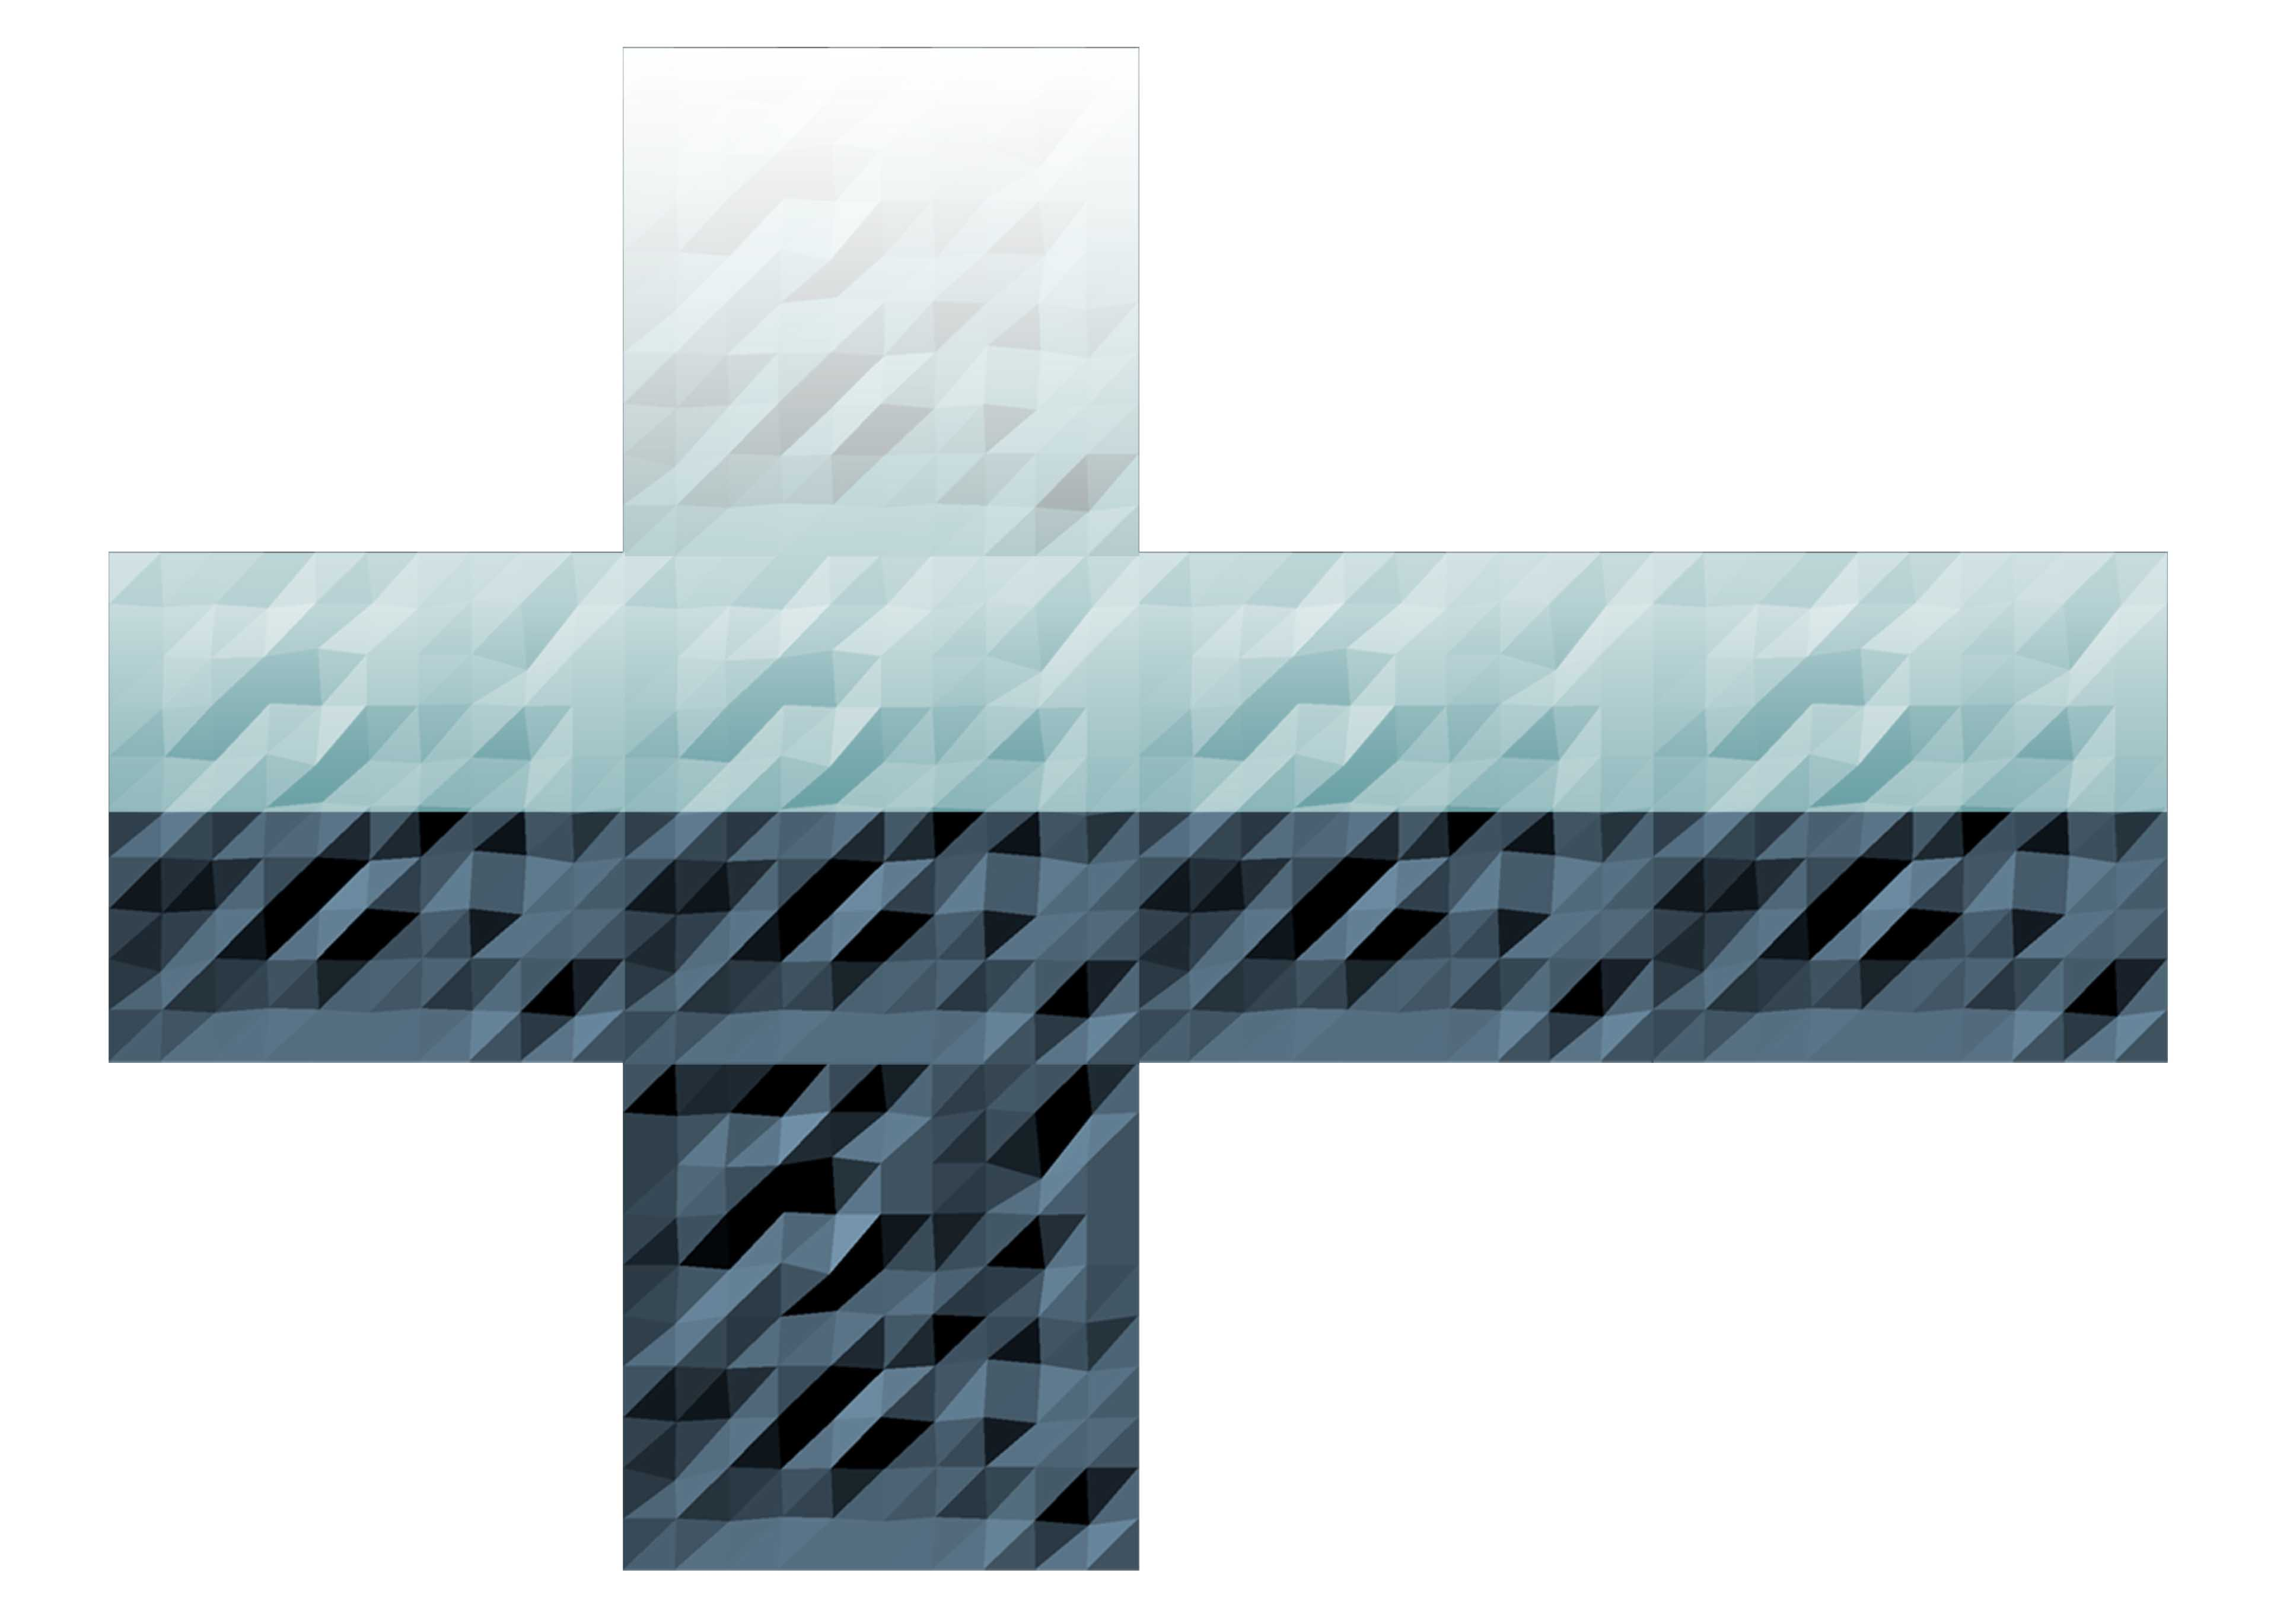
\includegraphics[width=0.8\textwidth]{images/Skybox}
	\caption{Screenshot der Skybox Textur}
	\label{fig:Skybox}
\end{figure}

Die Skybox (siehe Abbildung \ref{fig:Skybox}) soll den charakteristischen Low Poly Stil des Spiels widerspiegeln. Um diesen erfolgreich umzusetzen, muss ein Würfel in Cinema4D mit Hilfe des Modelling Tools bearbeitet und im Anschluss dessen Textur gebacken werden. Die Textur, welche in einer aufgeklappten Würfelform ausgegeben wird, kann dann in Photoshop nach coleriert werden.